% -*- mode: noweb; noweb-default-code-mode: R-mode; -*-
\documentclass[11pt]{article}
%% Set my margins
\setlength{\oddsidemargin}{0.0truein}
\setlength{\evensidemargin}{0.0truein}
\setlength{\textwidth}{6.5truein}
\setlength{\topmargin}{0.0truein}
\setlength{\textheight}{9.0truein}
\setlength{\headsep}{0.0truein}
\setlength{\headheight}{0.0truein}
\setlength{\topskip}{0pt}
%% End of margins

%%\pagestyle{myheadings}
%%\markboth{$Date$\hfil$Revision$}{\thepage}

\usepackage[pdftex,
bookmarks,
bookmarksopen,
pdfauthor={Bradley Efron, Balasubramanian Narasimhan},
pdftitle={Local FDR Simulation Example}]{hyperref}


\title{Local FDR Simulation Example}
\author{Bradley Efron and Balasubramanian Narasimhan\\
  Department of Statistics\\
  Stanford University\\ 
  Stanford, CA 94305}

\date{\today}



\usepackage{/home/depot/swtree/depot/R-2.0.1/lib/R/share/texmf/Sweave}
\begin{document}
%\VignetteIndexEntry{Local FDR}
%\VignetteKeywords{FDR, local FDR}
%\VignettePackage{locfdr}
\maketitle

\section{A Simulated Example}
This simulation example involves 2000 ``genes'', each of which has
yielded a test statistic $z_i$, with $z_i \approx N(mu_i, 1)$,
independently for $i=1,2,\ldots,2000$.

Here $mu_i$ is the ``true score'' of gene $i$, which we observe only
noisily. 1800 (90\%) of the $\mu$ values are zero; the remaining 200
(10\%) are from a $N(3,1)$ distribution. The data are contained in the
dataset \texttt{lfdrsim}, where the $z_i$ are the column \texttt{zex}.  

\begin{Schunk}
\begin{Sinput}
> library(locfdr)
> data(lfdrsim)
> zex <- lfdrsim[, 2]
\end{Sinput}
\end{Schunk}

A histogram shows that the $z_i$ have a long tail to the right of
zero, but with no obvious second mode near $z=3$.


\begin{Schunk}
\begin{Sinput}
> hist(zex, breaks = seq(-3.4, 7.2, 0.2), xlab = "z-value")
\end{Sinput}
\end{Schunk}
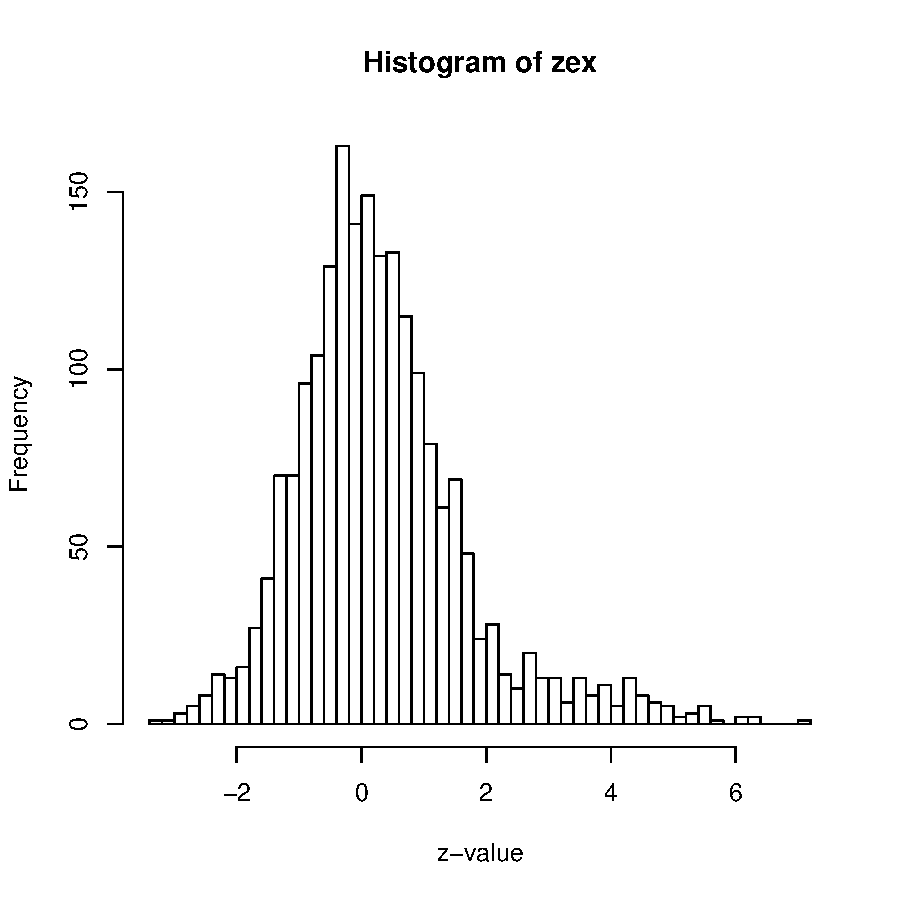
\includegraphics{locfdr-example-Histogram}

The \texttt{locfdr} package allows us to compute the fdr, the
individual fdr values for the 2000 genes, the descriptive vector
\texttt{f0.p0} and a $119\times 7$ matrix of results including the
local fdr. 

\begin{Schunk}
\begin{Sinput}
> w <- locfdr(zex)
\end{Sinput}
\begin{Soutput}
Loading required package: splines 
\end{Soutput}
\end{Schunk}

Let's examine \texttt{f0.p0}. 

\begin{Schunk}
\begin{Sinput}
> print(w$f0.p0)
\end{Sinput}
\begin{Soutput}
NULL
\end{Soutput}
\end{Schunk}

The above indicates that the empirical null $f_0(z)$ was estimated to
be $N(.0226,.979^2)$, and that the estimated proportion of null cases
is 0.916. (The fitting method is conservative in the sense of tending
to overestimate the true null proportion.) In this case the empirical
null has done a good job of estimating what we happen to know is the
true $N(0,1)$ null.

We now add the fdr plot to the histogram (scaled up by a factor of
100).

\begin{Schunk}
\begin{Sinput}
> hist(zex, breaks = seq(-3.4, 7.2, 0.2), xlab = "z-value", main = "Histogram of zex with 100.fdr")
> lines(w$mat[, 1], 100 * w$mat[, 2], lwd = 3)
\end{Sinput}
\end{Schunk}
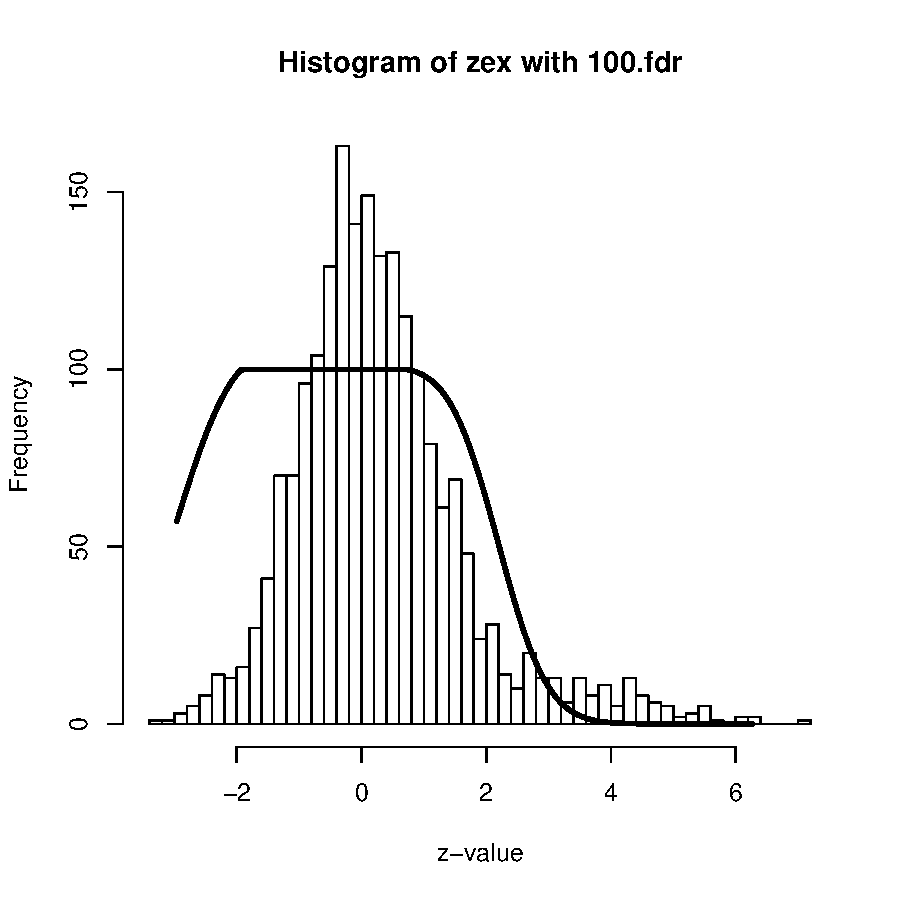
\includegraphics{locfdr-example-FDR-Plot}

This shows that the only small $fdr(z)$ values are on the right side, as
they should be, with $fdr(z)$ declining to zero as $z$ goes from 2 to
4. 

We can now compute $z$ such that $fdr(z)=0.2$.

\begin{Schunk}
\begin{Sinput}
> zp <- approx(w$mat[, 2], w$mat[, 1], 0.2)
> print(zp)
\end{Sinput}
\begin{Soutput}
$x
[1] 0.2

$y
[1] 2.791499
\end{Soutput}
\end{Schunk}

So, $fdr(2.79) = 0.2$. We now compute how many genes have fdr
less than $0.2$.

\begin{Schunk}
\begin{Sinput}
> sum(zex > zp$y)
\end{Sinput}
\begin{Soutput}
[1] 117
\end{Soutput}
\end{Schunk}

Thus, we have 117 genes with fdr less than .2. Of these 117, only 4
are actually Nulls, i.e. have $\mu_i=0$. This is in rough agreement
with the tail area Fdr, \texttt{Fdrleft}, which equals .041 at
$z=2.79$. The fact that the local fdr is nearly five times greater, .2
compared to .041, shows that genes near the boundary point 2.79 are
much more likely to be false discoveries than the average gene having
$z > 2.79$.

\end{document}
